\documentclass[tikz, border=5mm]{standalone}
\usepackage{tikz}
\usetikzlibrary{positioning, arrows.meta, calc}

\begin{document}
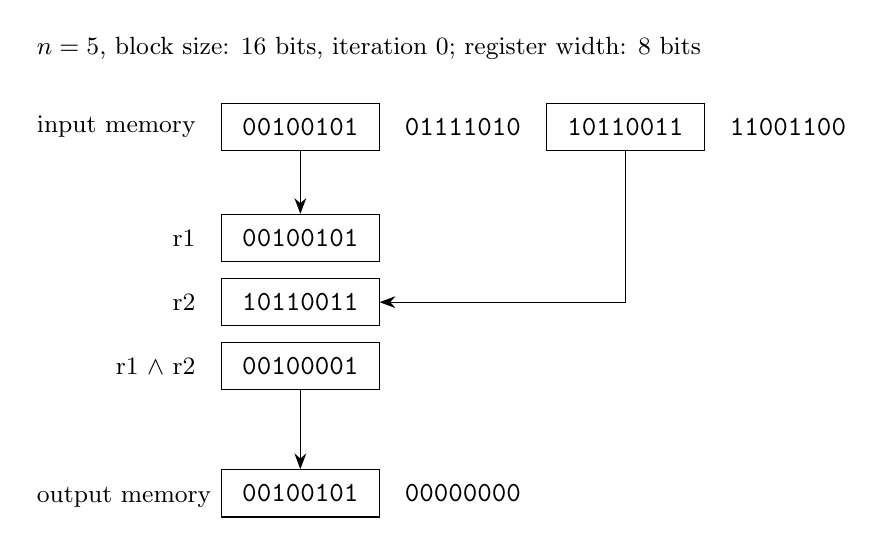
\begin{tikzpicture}[
    node distance=2mm and 5mm, % default vertical and horizontal node distance
    bitbox/.style={draw, font=\ttfamily, inner sep=2.5pt, minimum height=6mm, minimum width=20mm},
    labelstyle/.style={font=\small}
]

% Header text
\node (rw_def) [labelstyle] {\(n=5\), block size: 16 bits, iteration 0; register width: 8 bits};

% Input Memory line
\node (mem_label) [labelstyle, below=10mm of rw_def.west, anchor=west] {input memory};
\node (mem1) [bitbox, right=2mm of mem_label] {00100101};
\node (mem2) [bitbox, right=0.5mm of mem1, draw=none] {01111010}; % Second part of block 1
\node (mem3) [bitbox, right=0.5mm of mem2] {10110011};
\node (mem4) [bitbox, right=0.5mm of mem3, draw=none] {11001100}; % Second part of block 2

% Registers
\node (r1_val) [bitbox, below=8mm of mem1] {00100101};
\node (r1_label) [labelstyle, left=2mm of r1_val] {r1};

\node (r2_val) [bitbox, below=2mm of r1_val] {10110011};
\node (r2_label) [labelstyle, left=2mm of r2_val] {r2};

% AND operation result
\node (r1andr2_val) [bitbox, below=2mm of r2_val] {00100001};
\node (r1andr2_label) [labelstyle, left=2mm of r1andr2_val] {r1 $\land$ r2};

% Arrows from Input Memory to Registers
\draw[-{Stealth[length=2mm, width=1.5mm]}] (mem1.south) -- (r1_val.north);
\draw[-{Stealth[length=2mm, width=1.5mm]}] (mem3.south) |- (r2_val.east);

\node (output_mem_label) [labelstyle, below=47mm of mem_label.west, anchor=west] {output memory};
\node (output_mem1) [bitbox, below=10mm of r1andr2_val] {00100101};
\node (output_mem2) [bitbox, right=0.5mm of output_mem1, draw=none] {00000000}; % Second part of block 1
%\node (mem3) [bitbox, right=0.5mm of mem2] {10110011};
%\node (mem4) [bitbox, right=0.5mm of mem3, draw=none] {11001100}; % Second part of block 2

% --- MODIFIED SECTION FOR OUTPUT ---
% Remove the old output label node
% \node (output_label) [labelstyle, right=8mm of r1andr2_val] {output};

% Output Memory line
% Position the first memory box for the output. The value is the result of r1 & r2.
% The 'right=47mm of r1andr2_val' positions output_mem_val1 such that there's space for its label and the arrow.

% Arrow from AND result to the first register of Output Memory
\draw[-{Stealth[length=2mm, width=1.5mm]}] (r1andr2_val.south) -- (output_mem1);
% --- END OF MODIFIED SECTION ---

\end{tikzpicture}
\end{document}
